% \VignetteIndexEntry{Introduction to OLINgui}
% \VignetteDepends{OLINgui}
% \VignetteKeywords{Expression Analysis, Preprocessing}
% \VignettePackage{OLINgui}

\documentclass[a4paper,11pt]{article}
\usepackage{a4wide}
\title{Introduction to OLINgui}
\author{Matthias E. Futschik\\ Institute for Theoretical Biology,  Humboldt-University\\ URL: \textit{http://itb.biologie.hu-berlin.de/$\sim$futschik/software/R/OLIN}}
\usepackage{/usr/lib/R/share/texmf/Sweave}
\begin{document}
\maketitle
\tableofcontents

\section{Overview}
The package \emph{OLINgui} provides a graphical user interface for
visualisation, normalisation and quality testing of two-channel microarray data using the  functions of the OLIN package.  
The graphical interface is  based on Tk widgets using the R-TclTk interface by Peter Dalgaard. It also employs
some pre-made widgets from the Bioconductor-package tkWidgets  by Jianhua Zhang for
the selection of objects or files to be loaded. 

OLINgui provides a convenient interface to most functions of the OLIN package without restriction
of flexibility. An exception is the visualization, where default arguments for plotting 
are used. To fine-tune plots, the underlying plotting functions in the OLIN package
may be applied. Usage of OLINgui assumes existing \emph{marray} objects for the batch of arrays to 
be analysed and normalised.  (For construction of \emph{marray} objects using a graphical interface, the reader is referred
 to the \emph{marrayInput} package.) Additionally to the  \emph{marray} object, 
some functions require an additional list of X- and Y-coordinates of spots. 
This list  has to be built \emph{by hand} yet. However, most functions of the OLIN package 
 do not require this list.  

A brief introduction to the  functionality of \emph{OLINgui} will be given in section 3.
For more details about the computational approaches, please refer to the OLIN package documentation
and the reference~\cite{toni}. 


%%%%%%%%%%%%%%%%%%%%%%%%%%%%%%%%%%%%%%%%%%%%%%%%%%%%%%%%%%%%%%%%%%%%%%%%%%%%%%%%
%%%%%%%%%%%
\section{Installation requirements}
Following software is required to run the OLINgui-package:
\begin{itemize} 
\item  R (>= 2.0.0). For installation of R, refer to \textit{http://www.r-project.org}.
\item  R-packages: methods, stat, locfit, tcltk. For installation of these add-on packages, refer to \textit{http://cran.r-project.org}.
\item Bioconductor packages: Biobase, marray, OLIN (>= 1.4.0). Refer to \textit{http://www.bioconductor.org} for installation. 
\end{itemize}

If all requirements are fulfilled, the OLINgui add-on R-package can be installed.\
 To see how to install add-on R-packages on your computer system, start \textit{R} 
and type in \textit{help(INSTALL)}.
Optionally, you may use the R-function \textit{install.packages()}. 
Once the OLINgui package is installed, you can load the package by 

\begin{Schunk}
\begin{Sinput}
> library(OLINgui)
\end{Sinput}
\end{Schunk}




\section{Functionality}

To start the graphical interface, type: 


\vspace{4mm}
\noindent \texttt{> OLINgui()}
\vspace{4mm}





A TclTk-Widget is launched (fig.1). The use of the interface is intuitive. The
GUI is divided into four sections; the order of these sections reflects the order
of a standard analysis and normalisation  procedure for a  microarray data set:
\begin{enumerate}
\item Loading of data set
\item Visualisation for data inspection
\item Application of statistical tests to identify experimental bias
\item Normalisation and scaling of data 
\end{enumerate} 

Note that only one data set at a time can be analysed or normalised. To visualise
or test the normalized data set, it is necessary to save/export this data set and
reload it. 

The general structure of the GUI is straight-forward.  Each button corresponds to a function in the OLIN package. 
If additional arguments for the function are needed,
 an input  window is launched.
Note that not everything will be checked to be of correct type.
 While some checks are implemented (e.g. checks if the loaded data set
has the correct class), most arguments remained unchecked before the underlying 
function is called (e.g. it will not be checked if the array index is a positive integer.)
If errors are produced, the validity of the input arguments should be examined.
For details about the required types of arguments and corresponding functions, please refer to the help pages of the OLIN package. In the following section, a brief introduction to
the functionality of OLINgui is given. As an example, the datasets \textit{sw} and
\textit{sw.xy} can be loaded in the global environment by

\begin{Schunk}
\begin{Sinput}
> data(sw)
> data(sw.xy)
\end{Sinput}
\end{Schunk}
and subsequently loaded for analysis using the \fbox{Browse objects} buttons.

   
\begin{figure}
\centering
\centering
\resizebox{0.5\textwidth}{!}{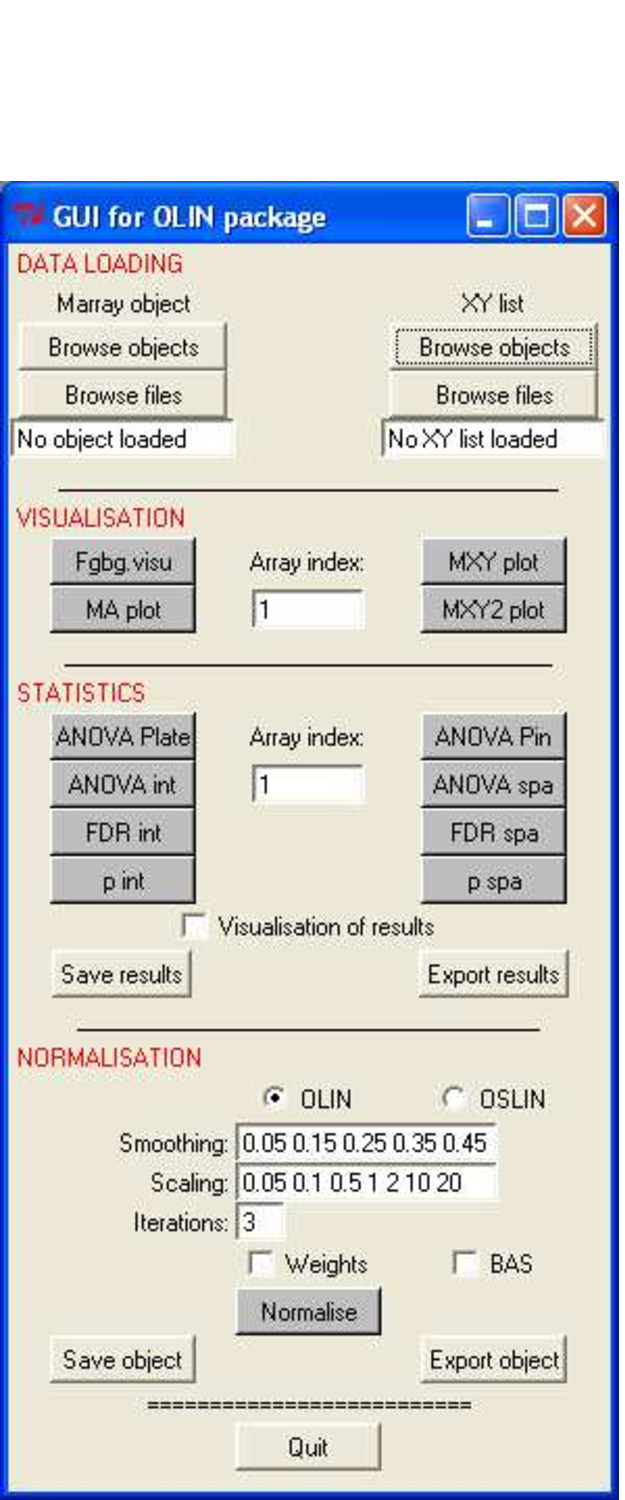
\includegraphics{OLINguiScreenshot.pdf}}
\caption{Screen-shot of OLINgui (version 1.0.1)}
\label{fgbg}
\end{figure}



\subsection{Loading data}

\textbf{Marray object}
\begin{itemize}
\item \fbox{Browse objects} Import of an Marray object of class \textit{marrayRaw}
 or \textit{marrayNorm} from the global environment (\textit{.GlobalEnv}). 
A window produced by the function \texttt{objectBrowser} of the 
tkWidgets package is generated. Note that, although
several objects can be selected, only the first selected object will be loaded. 
A check is performed if the object to be loaded belongs to the correct classes. 

\item \fbox{Browse file} Loading of an R data set   of class \textit{marrayRaw}
 or \textit{marrayNorm} stored in a file. 
A window produced by the function \texttt{fileBrowser} of the 
tkWidgets package is generated. Note that, although
several files can be selected, only the first selected file is loaded. A check is performed if the object to be loaded belongs to the correct classes. 
\end{itemize}

\noindent \textbf{XY  list}
\begin{itemize}
\item \fbox{Browse objects} Loading of an R object of type \textit{list} from the global environment (\textit{.GlobalEnv}). 
A window produced by the function \texttt{objectBrowser} of the 
tkWidgets package is generated. Note that, although
several objects can be selected, only the first selected object is loaded. A check is performed if the object is of type \textit{list} with name attributes ``X'' and ``Y''. No
check is performed if the dimensions of the list elements are correct.


\item \fbox{Browse file} Loading of an R object of type \textit{list} stored in a file. 
A window produced by the function \texttt{fileBrowser} of the 
tkWidgets package is generated. Note that, although
several objects can be selected, only the first selected object is loaded. A check is performed if the object is of type \textit{list} with name attributes ``X'' and ``Y''. No
check is performed if the dimensions of the list elements are correct.

\end{itemize}

The names of the marray object and XY list are shown in the text fields below the buttons.



\subsection{Visualisation}

\begin{itemize}
\item \textit{Array index:} Selection of the arrays to be visualised. If several arrays are to
be visualised, the indeces have to  be space delimited. If no array index is given, all
arrays of the data set will  be visualised.
 
\item \fbox{Fgbg.visu} Call of the function \texttt{fgbg.visu}. Visualisation of spatial  
 distribution of foreground and background fluorescence  intensities in both channels.

\item \fbox{MA plot} Produces  MA-plots that  display the logged fold change 
($M=log_{2}(Ch2) - log_{2}{Ch1}$) with respect to the average logged spot intensity  ($A=0.5(log_{2}(Ch1) + log_{2}{Ch2})$).

\item \fbox{MXY plot} Call of the function \texttt{mxy.plot}. Visualisation of spatial distribution of logged fold change ($M$) across the array. The row and column indeces are used
as proxies for the spatial spot coordinates.

\item \fbox{MXY2 plot} Call of the function \texttt{myx2.plot}. Visualisation of spatial distribution of logged fold change ($M$) across the array. In contrast to \texttt{mxy.plot},
function \texttt{mxy2.plot} produces MXY-plots based on spatial spot coordinates as stored
in the XY-list. Therefore, this function requires that a XY-list has been loaded. 


\end{itemize}

\subsection{Statistics}


\begin{itemize}
\item \textit{Array index:} Selection of the arrays to be analysed. If several arrays are to
be analysed, their indeces should be space delimited. If no array index is given, all
arrays of the data set will be  analysed. 

\item \fbox{ANOVA Plate}  Call of the function \texttt{anovaplate}. An one-factorial ANOVA assessing plate-dependent bias is performed. If \textit{Visualisation of results} is ticked, a window
with the results is shown. 


\item \fbox{ANOVA Pin} Call of the function \texttt{anovapin}. An one-factorial ANOVA assessing pin-dependent bias is performed. If \textit{Visualisation of results} is ticked, a window
with the results is shown. 

\item \fbox{ANOVA int}  Call of the function \texttt{anovaint}. An one-factorial ANOVA assessing intensity-dependent bias is performed. The predictor variable is $A$; the response variable is $M$.  The number of intervals along the A-axis
has to be chosen. This gives the number of factors for the ANOVA.  
If \textit{Visualisation of results} is ticked, a window with the results will be shown. 

\item \fbox{ANOVA spa}  Call of the function \texttt{anovaspatial}. An  one-factorial 
ANOVA assessing spatial bias is performed. The array is spatially divided in a number of rectangular blocks
determining the factors for the ANOVA. The predictor variable is the index of the spatial blocks; the response variable is $M$. The number of blocks can be selected  by the input arguments determining the number
of intervals in the X and Y direction.   If \textit{Visualisation of results} is ticked, 
the  results will be shown. Additionally, \
 a plot is produced showing the significance of blocks based on the ANOVA model. 

\item \fbox{FDR int}  Call of the function \texttt{fdr.int}. This function assesses
 the intensity-dependent dye bias using two one-sided permutation tests. The test statistics is the average value 
of  $M$  in a spot intensity neighourhood of chosen size. The significance (given by the false discovery
rate) indicates the probability of observing the actual average values  $\bar{M}$ 
assuming $A$ and $M$ are independent. 
 The number of permutations determines how often
the  intensity order of spots  is permutated for the calculation of the
 empirical background distribution.
For averaging, \textit{mean} or \textit{median} can be chosen.
 If \textit{Visualisation of results} is ticked,  a plot is produced showing the false discovery rates for the corresponding
 intensity neighbourhoods. Green (red)  dots indicate the false discovery rate 
for  negative (positive) derivations of the test statistics.
 Low false discovery rates indicate
intensity-dependent bias.  Note, however, that the scale of the y-axis  is $-log_{10}$(fdr) in both directions.
 

\item \fbox{FDR spa}  Call of the function \texttt{fdr.spatial}.The function assesses location-dependent dye bias using 
one-sided  permutation tests. 
The number of permutations determines how often the spatial location of spots on  an array is permutated for the calculation of the empirical background distribution.    
If \textit{Visualisation of results} is ticked, 
a MXY plot is generated  showing the false discovery rate for  $\bar{M}$  of  spatial spot 
neighbourhoods for positive (red) and negative (green) deviations. 

\item \fbox{p int}  Call of the function \texttt{p.int}. This function assesses intensity-dependent dye bias using a randomisation test. Similarly to \textit{fdr.int}, the average logged fold change ($\bar{M}$) in a spot intensity neighourhood is compared to 
a empirical background distribution based on randomised intensity orders of spots.  
The number of samples determines how many random samples (with replacement) are generated  
for the construction of an empirical background distribution.   
The significance of  $\bar{M}$ is  based on Fisher's  test. Several methods for p-value adjustment can be chosen.
If  \textit{Visualisation of results} is ticked, the significance is plotted along the spot intensity axis.  Green (red)  dots indicate the false discovery rate 
for  negative (positive) deviations of the test statistics.
 Low false discovery rates indicate
intensity-dependent dye bias.  Note, however, that the scale of the y-axis  is $-log_{10}$(fdr).
 
  

\item \fbox{p spa}  Call of the function \texttt{p.spatial}. This function assesses location-dependent dye bias using a randomisation test.  The number of samples determines how many random 
samples (with replacement) are generated  for the construction of an empirical background distribution.   
Note that the difference between number of samples and number of permutations used for \texttt{fdr.int}.
The latter refers to the whole data set. 
The significance of  $\bar{M}$ is  based on Fisher's test. Several methods for p-value adjustment can be chosen.
If \textit{Visualisation of results} is ticked, 
a MXY plot is generated  showing the significance of  $\bar{M}$  for spatial spot 
neighbourhoods. 

\item \textit{Visualisation of results}: Results are visualised if checkbutton is ticked.

\item \fbox{Save results}  The results are stored in a list and saved to a file. Each list elements corresponds to
the output of the underlying functions that has been used for the statistical analysis.  

\item \fbox{Export results}  The results are stored in a list and exported to the global environment.
 Each list elements corresponds to
the output of the underlying functions that has been used for the statistical analysis.  



\end{itemize}


\subsection{Normalisation}
\begin{itemize}
\item \textit{IN, OIN, LIN, OLIN, OSLIN radiobuttons}: Selection which normalisation scheme should be applied. For
a description of these methods, see the \emph{OLIN help pages}.


\item \textit{Smoothing}: Smoothing parameter(s) to be used or tested for  normalisation. It can be any 
value between 0 and 1. Values close to 0, however, may produce unstable normalisation results. 
The input  should be a scalar for IN and LIN. This value is then used for local regression. 
It can be a space-delimited list for OIN, OLIN and OSLIN. These values are tested in the GCV procedure
with the optimal smoothing parameter used subsequently for normalisation.     

\item \textit{Scaling}: Scaling parameter(s) to be used or tested  for location-dependent normalisation.
The scaling  parameter determines the amount of smoothing in Y-direction compared to smoothing
in X-direction. It is used for LIN/OLIN/OSLIN. The input can be a single value for LIN. Alternatively,
\emph{TRUE} or \emph{FALSE} can be chosen. The input value \emph{TRUE} leads to scaling by the standard 
deviation. No scaling is performed for the value \emph{FALSE}. 
For OLIN or OSLIN, a list of values should be given. 

\item \textit{Iterations}: Number of iterations in the  LIN/OLIN/OSLIN procedure. Three are usually sufficient. 

\item \textit{Weights}: Weighting of spots for local regression. If the checkbutton is ticked,
spots are weighted by the weights stored in \textit{maW} slot of the marray object.

\item \textit{BAS}: Subsequent between-array normalisation (scaling). If the checkbutton is ticked,
a between-array normalisation is applied. Three methods can be chosen from: \textit{Var}- arrays
are scaled to have the same variance of $M$,   \textit{Mad} - arrays are scaled to have the same
median absolute deviation of $M$ and \textit{QQ} - arrays are scaled using quantile normalisation. 

\item \fbox{Normalise}: Call of the function \texttt{olin}.

\item \fbox{Save object}: The normalised batch of arrays will be stored as maNorm object and saved to a file.


\item \fbox{Export object}: The normalised batch of arrays will be exported to the global environment.

\end{itemize}

To visually inspect and statistically test 
the results of the normalisation, the normalised data has to be exported (or saved) and reloaded. 

%BIBLIOGRAPHY
\begin{thebibliography}{99}
\bibitem{toni} M.Futschik and T. Crompton (2004) Model selection and efficiency testing for normalisation of cDNA microarray data, \emph{Genome Biology}, 5:R60  


\end{thebibliography}

\end{document}

